%This template is based on one provided by the American Physical Society for submission to its journals.

\documentclass[aps,twocolumn,preprintnumbers]{revtex4}

%The following packages add LaTeX commands that make formatting and writing math easier

\usepackage{graphicx}  % Include figure files
\usepackage{subfigure}
\usepackage{multirow}

\linespread{1.1}
\usepackage{fancyhdr}
\usepackage{longtable}
\usepackage{parskip}
\usepackage[T1]{fontenc}
\usepackage{dcolumn}   % Align table columns on decimal point

\usepackage{bm}        % bold math
\usepackage{amsfonts}  % Common math fonts
\usepackage{amsmath}   % Common math functions
\usepackage{amssymb}   % Common math symbols
\usepackage{url}
\usepackage{physics}
%The following custom commands simplify commonly used LaTeX commands

\newcommand{\pic}[2]{
  \begin{center} \includegraphics[scale=#1]{#2}
\end{center}}
\newcommand{\re}[1]{\mathrm{Re}\left(#1\right)}
\newcommand{\im}[1]{\mathrm{Im}\left(#1\right)}
\newcommand{\bdot}[1]{\dot{ \bb {#1}}}
\newcommand{\bddot}[1]{\ddot{ \bb {#1}}}
\newcommand{\bidot}[1]{\dot{ \bi{ #1}}}
\newcommand{\biddot}[1]{\ddot{ \bi {#1}}}
\newcommand{\ep}{\varepsilon}
\newcommand{\for}{\quad \quad \mathrm{for} \quad\quad}
\newcommand{\then}{\quad \quad \implies \quad\quad}
\newcommand{\an}{\quad \quad \mathrm{and} \quad\quad}
\newcommand{\ifff}{\quad \quad \mathrm{if} \quad\quad}
\newcommand{\where}{\quad \quad \mathrm{where} \quad\quad}
\newcommand{\dg}{^\dagger}
\newcommand{\semi}{\quad \quad \mathrm{;} \quad\quad}
\newcommand{\paren}[1]{\left( #1 \right)}
\newcommand{\brac}[1]{\left[ #1 \right]}
\newcommand{\bra}[1]{\left\langle #1 \right|}
\newcommand{\exv}[1]{\left\langle #1 \right\rangle}
\newcommand{\pwisein}{\left\{
  \begin{array}{ll}}
    \newcommand{\pwiseout}{
  \end{array}\right.}
  \newcommand{\ket}[1]{\left| #1 \right\rangle}
  \newcommand{\bracket}[2]{\left\langle #1 | #2 \right\rangle}
  \newcommand{\trace}[1]{\mathrm{Tr} \left( #1 \right)}
  \renewcommand{\det}[1]{\mathrm{det}\left( #1 \right)}
  \newcommand{\del}[1]{\frac{\partial}{\partial #1}}
  \newcommand{\fulld}[1]{\frac{d}{d #1}}
  \newcommand{\fulldd}[2]{\frac{d #1}{d #2}}
  \newcommand{\dell}[2]{\frac{\partial #1}{\partial #2}}
  \newcommand{\delltwo}[2]{\frac{\partial^2 #1}{\partial #2 ^2}}
  \newcommand{\bb}{\mathbf}
  \newcommand{\bi}{\boldsymbol}
  \newcommand{\eq}[1]{
    \begin{equation} #1
  \end{equation}}
  \newcommand{\radhalf}{ \frac{ \sqrt{2}}{2}}
  \newcommand{\sigx}{\left(
      \begin{array}{cc} 0 & 1\\ 1 & 0
  \end{array}\right)}
  \newcommand{\sigy}{\left(
      \begin{array}{cc} 0 & -i\\ i & 0
  \end{array}\right)}
  \newcommand{\sigz}{\left(
      \begin{array}{cc} 1 & 0\\ 0 & -1
  \end{array}\right)}
  \renewcommand{\matrix}[1]{\left(
      \begin{array} #1
  \end{array}\right)}
  \newcommand{\thermo}[3]{\left( \frac{\partial #1}{\partial #2} \right)_{#3}}
  \newcommand{\coolfrac}[2]{\left( \frac{ #1}{ #2} \right)}

  \setlength{\parindent}{10pt}

  \begin{document}

  \title{Aplicación del método de Hartree-Fock para obtener numéricamente las energías y orbitales del átomo de Helio}

  \author{Jovanny Jara}

  \affiliation {\it Instituto de Física y Astronomía, Universidad de Valparaíso}

  \date{\today}

  \begin{abstract}

    El trabajo presenta una implementación numérica de alto rendimiento en C/CUDA para resolver el átomo de Helio desde primeros principios, utilizando la aproximación de Hartree-Fock en una discretización de espacio real (Real-Space Grid). El algoritmo se basa en el método de Propagación en Tiempo Imaginario (ITP) implementado mediante la técnica Split-Operator para resolver la ecuación de Schrödinger, aprovechando la arquitectura masivamente paralela de una GPU para procesar mallas de alta resolución ($256^3$ puntos).

    La simulación del estado fundamental ($1s2$) convergió a una energía total de -78.408 eV, presentando una discrepancia de apenas $0.69\%$ respecto al límite teórico Hartree-Fock. Adicionalmente, se logró estabilizar y visualizar estados excitados con simetrías p y d mediante la imposición de imetrías, obteniendo configuraciones doblemente excitadas consistentes con el modelo restringido (RHF). Los resultados validan la eficacia de los métodos en malla en GPU como una alternativa precisa y flexible a los métodos tradicionales de conjuntos de base para la simulación cuántica.

  \end{abstract}

  \maketitle

  \section{Introducción}

  %P1: Intro: scientific motivation

  Los sistemas cuánticos de dos cuerpos, como el átomo de Hidrógeno, son sistemas que poseen solución analítica. Sin embargo, al tener tres o más particulas, como el átomo de Helio, ya no es posible encontrar una solución analítica debido a que resolver la ecuación de Schrödinger para N electrones requiere obtener una solución a una función de 3N coordenadas.
  %P2: More intro: approach, definitions, history, context, rationale

  Específicamente para el átomo de Helio, la dificultad surge de la repulsión electrónica entre los electrones, un término que acopla las ecuaciónes diferenciales a resolver y obliga a utilizar aproximaciones aplicando métodos numéricos para obtener una solución.

  %P3: What you did, what you found

  Una forma de abordar esta complejidad es reducir el problema de N cuerpos a N problemas de un solo cuerpo, aproximando la función de onda total como un producto de funciones de onda de un solo electrón. Esto transforma efectivamente el problema a un problema de electrón independiente.

  Esta aproximación generalmente ignora la correlación electrónica; los electrones pueden ocupar el mismo sitio, por lo que el movimiento de cada uno no está limitado por el otro. Esto conlleva a un error significativo y es necesario aplicar métodos de aproximación mas avanzados como el método de Hartree-Fock o de campo auto-consistente (SCF), método iterativo que no considera la correlación completamente, pero si considera la repulsión entre los electrones, entregando una buena aproximación a la solución.

  \section{Teoría}

  \subsection{Método de Hartree-Fock (SCF)}

  Buscamos resolver la ecuación de Schrödinger independiente del tiempo (TISE) para el átomo de Helio dada por

  \begin{equation}
    \hat{H} \psi(\bm{\mathrm{r}}_1,\bm{\mathrm{r}}_2) = E\psi(\bm{\mathrm{r}}_1,\bm{\mathrm{r}}_2)
  \end{equation}

  Donde tenemos el siguiente Hamiltoniano

  \begin{multline}
    \hat{H}_{He} = \frac{\hbar^2}{2m_e}\left(-\nabla_1^2 -\nabla_2^2\right) \\- \frac{e^2}{4\pi\epsilon_0}\left(\frac{2}{r_1} + \frac{2}{r_2} + \frac{1}{|\bm{\mathrm{r}}_2-\bm{\mathrm{r}}_1|}\right)
  \end{multline}

  El cual puede ser reescrito en unidades atómicas, quedando

  \begin{equation}
    \hat{H}_{He} = -\frac{1}{2}\left(\nabla_1^2 + \nabla_2^2\right) - 2\left(\frac{1}{r_1} + \frac{2}{r_2}\right) + \frac{1}{|\bm{\mathrm{r}}_2-\bm{\mathrm{r}}_1|}
  \end{equation}

  En el método de Hartree-Fock\cite{udel_hf}, se realiza una aproximación de la función de onda como un producto de orbitales independientes, donde cada orbital depende de la posición de cada electron y tiene asociada una sola energía orbital. Para el Helio tenemos entonces

  \begin{equation}
    \chi(\bm{\mathrm{r}}_1,\bm{\mathrm{r}}_2) = \phi(\bm{\mathrm{r}}_1)\phi(\bm{\mathrm{r}}_2)
  \end{equation}

  Como se desconoce la forma de estos orbitales, los podemos etiquetar como $\phi^{HF}(\bm{\mathrm{r}}_1)$ y $\phi^{HF}(\bm{\mathrm{r}}_2)$. Estos son los orbitales de Hartree-Fock.

  La independencia de los orbitales, sin embargo, no es estricta en el método: se considera que cada electrón interactúa con la densidad de carga del otro, es decir, un potencial promedio generado por la densidad de carga.

  Si describimos dicha densidad de carga en unidades atómicas para el segundo electrón, por ejemplo, como

  \begin{equation}
    \rho(\bm{\mathrm{r}}_2) = \phi^*(\bm{\mathrm{r}}_2) \phi(\bm{\mathrm{r}}_2) = |\phi(\bm{\mathrm{r}}_2)|^2
  \end{equation}

  podemos entonces escribir un potencial efectivo para el primer electron al integrar la interacción coulombiana dada por esta densidad de carga. Esto es, un potencial coulombiano percibido por el primer electrón promediado sobre todas las posiciones del segundo electrón. En efecto

  \begin{equation}
    U_1^{eff}(\bm{\mathrm{r}}_1) = \int\phi^*(\bm{\mathrm{r}}_2)\frac{1}{|\bm{\mathrm{r}}_2-\bm{\mathrm{r}}_1|}\phi(\bm{\mathrm{r}}_2)\mathrm{d}\bm{\mathrm{r}}_2
  \end{equation}

  Con esto podemos escribir un Hamiltoniano efectivo para el primer electrón

  \begin{equation}
    \hat{H}_1^{eff}(\bm{\mathrm{r}}_1) = -\frac{1}{2}\nabla_1^2 - \frac{2}{r_1} + U_1^{eff}(\bm{\mathrm{r}}_1)
  \end{equation}

  Y también una ecuación de Schrödinger reducida para el primer electrón

  \begin{equation}\label{eq:tise}
    \hat{H}_1^{eff}(\bm{\mathrm{r}}_1)\phi^{HF}(\bm{\mathrm{r}}_1) = \epsilon_1\phi^{HF}(\bm{\mathrm{r}}_1)
  \end{equation}

  Así, obtenemos la funcion de onda para el primer electrón, lo que nos permite encontrar una nueva función para el segundo electrón realizando los mismos pasos. Este es el método SCF, mejor descrito a continuación.

  \begin{itemize}
    \item Proponer función de prueba para $\phi(\bm{\mathrm{r}}_2)$
    \item Usar $\phi(\bm{\mathrm{r}}_2)$ para calcular $U_1^{eff}(\bm{\mathrm{r}}_1)$
    \item Resolver la ec. (\ref{eq:tise}) para encontrar $\phi(\bm{\mathrm{r}}_1)$
    \item Usar $\phi(\bm{\mathrm{r}}_1)$ para calcular  $U_2^{eff}(\bm{\mathrm{r}}_2)$
    \item Resolver (\ref{eq:tise}) para encontrar un nuevo $\phi(\bm{\mathrm{r}}_2)$
    \item Continuar las iteraciones hasta alcanzar convergencia auto-consistente, es decir, que las funciones de onda dejen de cambiar en las siguientes iteraciones.
  \end{itemize}

  Con esto, se tiene entonces la solución completa a la ecuación de Schrödinger como

  \begin{equation}
    \chi(\bm{\mathrm{r}}_1,\bm{\mathrm{r}}_2) = \phi^{HF}(\bm{\mathrm{r}}_1)\phi^{HF}(\bm{\mathrm{r}}_2)
  \end{equation}

  Podemos entonces encontrar la energía total del sistema o la energía de Hartree-Fock mediante el principio variacional, el cual establece

  \begin{equation}
    E_{var} = \frac{\smallint\chi^*\hat{H}\chi\mathrm{d}\bm{\mathrm{r}}}{\smallint\chi^*\chi\mathrm{d}\bm{\mathrm{r}}} = \int\chi^*\hat{H}\chi\mathrm{d}\bm{\mathrm{r}}
  \end{equation}

  Donde la ultima igualdad asume que la función de onda, y por lo tanto la función de prueba, está normalizada. Entonces, la energía de Hartree-Fock

  \begin{align}
    E^{HF} &= \int\chi^*(\bm{\mathrm{r}}_1,\bm{\mathrm{r}}_2)\hat{H}_{He}\chi(\bm{\mathrm{r}}_1,\bm{\mathrm{r}}_2)\mathrm{d}\bm{\mathrm{r}}_1\mathrm{d}\bm{\mathrm{r}}_2\\
    &= I_1 + I_2 + J_{12}
  \end{align}

  Donde tenemos los términos

  \begin{align}
    I_1 &= \int\phi^{HF*}(\bm{\mathrm{r}}_1)\left[-\frac{\nabla_1^2}{2} -\frac{2}{r_1}\right]\phi^{HF}(\bm{\mathrm{r}}_1)\mathrm{d}\bm{\mathrm{r}}_1\\
    I_2 &= \int\phi^{HF*}(\bm{\mathrm{r}}_2)\left[-\frac{\nabla_2^2}{2} -\frac{2}{r_2}\right]\phi^{HF}(\bm{\mathrm{r}}_2)\mathrm{d}\bm{\mathrm{r}}_2\\
    J_{12} &= \int\chi^*(\bm{\mathrm{r}}_1,\bm{\mathrm{r}}_2)\frac{1}{|\bm{\mathrm{r}}_2-\bm{\mathrm{r}}_1|}\chi(\bm{\mathrm{r}}_1,\bm{\mathrm{r}}_2)\mathrm{d}\bm{\mathrm{r}}_1\mathrm{d}\bm{\mathrm{r}}_2
  \end{align}

  Podemos dejar expresada la energía del sistema en términos de las energías de los orbitales viendo que:

  \begin{align}
    \hat{H}_1^{eff}(\bm{\mathrm{r}}_1)\phi^{HF}(\bm{\mathrm{r}}_1) &= \epsilon_1\phi^{HF}(\bm{\mathrm{r}}_1)\\
    \epsilon_1 &= \int\phi^{HF*}(\bm{\mathrm{r}}_1)\hat{H}_1^{eff}\phi^{HF}(\bm{\mathrm{r}}_1)\mathrm{d}\bm{\mathrm{r}}_1\\
    &= I_1 + J_{12} = E^{HF} - I_2 \\
    \implies \epsilon_2 &= E^{HF} - I_1
  \end{align}

  Luego, si hacemos

  \begin{equation}
    \epsilon_1 + \epsilon_2 = I_1 + I_2 + 2J_{12} = E^{HF} - J_{12}
  \end{equation}

  Por lo tanto, la energía total

  \begin{equation}
    E^{HF} = \epsilon_1 + \epsilon_2 - J_{12}
  \end{equation}

  Es importante recalcar que el método de Hartree-Fock, al ser una aproximación de campo medio, posee un límite intrínseco en la precisión de la energía que puede calcular. El valor exacto de la energía del estado fundamental del átomo de Helio, determinado experimentalmente, es $E_{exp} = -79.00$ eV \cite{nist}.

  Sin embargo, la mejor energía posible obtenible por este método (el Límite Hartree-Fock) es $E{HF} =-77.87$ eV.

  Esta diferencia es la energía de correlación, que el método SCF no considera.

  \subsection{Propagación por Tiempo Imaginario (ITP) y Método Split-Operator (SOM)}

  Si bien el método de Hartree-Fock nos permite encontrar funciones de onda para sistemas de múltiples electrones, de igual forma exige resolver la ecuación de Schrödinger. Un buen método para ello es el de propagación por tiempo imaginario o ITP \cite{lehtovaara}.

  El método ITP considera la ecuación de Schrödinger dependiente del tiempo (TDSE). En unidades atómicas:

  \begin{equation}\label{eq:tdse}
    i \frac{\partial}{\partial t}\Psi(\bm{\mathrm{r}}, t) = \hat{H}\Psi(\bm{\mathrm{r}}, t)
  \end{equation}

  cuya solución general se escribe

  \begin{equation}
    \Psi(\bm{\mathrm{r}}, t) = e^{-i\hat{H}t}\Psi(\bm{\mathrm{r}}, 0) =\sum_n c_n \phi_n(\bm{\mathrm{r}})e^{-iE_nt}
  \end{equation}

  Si hacemos un cambio de variable llamado rotación de Wick, donde

  \begin{equation}
    t = -i\tau
  \end{equation}

  Y reemplazamos en (\ref{eq:tdse}), ahora la solución general queda de la siguiente forma

  \begin{equation}
    \Psi(\bm{\mathrm{r}}, \tau) = e^{-\hat{H}\tau}\Psi(\bm{\mathrm{r}}, 0) =\sum_n c_n \phi_n(\bm{\mathrm{r}})e^{-E_n\tau}
  \end{equation}

  La gracia de aplicar esta rotación es convertir el operador de evolucion temporal unitario $\hat{U}(t) \equiv e^{-i\hat{H}t}$ a un operador de tiempo imaginario difusivo $\hat{U}(\tau) \equiv e^{-\hat{H}\tau}$, transformando la solución oscilatoria en una difusiva.

  Asumiendo que existe un estado fundamental con energía $E_0$, los estados excitados tienen energías $E_i > E_0$ por lo que, al propagar el tiempo imaginario al infinito, estos términos decaen exponencialmente más rapido que el estado base, es decir

  \begin{equation}
    \lim_{\tau \to \infty} \Psi(\bm{\mathrm{r}}, \tau) \propto \Psi_0(\bm{\mathrm{r}})
  \end{equation}

  Esto es, en escencia, un filtro que busca aislar el estado fundamental, que converge al autoestado con la energía mas baja.

  Como se desea aplicar numéricamente el método, es relevante considerar que evaluar directamente la exponencial con el hamiltoniano es muy complicado generalmente, por lo que es conveniente reescribir el operador en su forma $\hat{H} = \hat{T} + \hat{V}$. Sin embargo, al escribir el hamiltoniano de esa forma los operadores no conmutan, por lo que no es posible escribir la exponencial como un producto, es decir:

  \begin{equation}
    e^{-(\hat{T} + \hat{V})t} \neq e^{-\hat{T}t}e^{-\hat{V}t}
  \end{equation}

  Aquí debemos aplicar la expansion de Suzuki-Trotter \cite{hatano_suzuki} al operador de tiempo imaginario. Para nuestro caso, conviene aplicar la expansión en segundo orden, quedando así el operador de la forma

  \begin{equation}
    \hat{U}(\tau) = e^{-\frac{\hat{V}}{2}\tau}e^{-\hat{T}\tau}e^{-\frac{\hat{V}}{2}\tau} + \mathcal{O}(\tau^3)
  \end{equation}

  Esta técnica de evolución temporal se conoce como método Split-Operator (SOM), dando a lugar el algoritmo de Propagación por Tiempo Imaginario mediante Operador Dividido (IT-SOM). De esta forma, al ser IT-SOM un método iterativo, al evolucionar la funcion de onda en pequeños pasos temporales $\Delta\tau$, tenemos por cada paso de evolución $n\to n+1$

  \begin{equation}
    \Psi^{(n+1)}(\bm{\mathrm{r}}, \Delta\tau) = \hat{U}(\Delta\tau)\Psi^{(n)}
  \end{equation}

  Por último, debemos tener en cuenta que el operador de tiempo imaginario no es unitario y provoca un decaimiento exponencial. Para prevenir que la funcion de onda se desvanezca es necesario renormalizarla en cada iteración:

  \begin{equation} \label{eq:som}
    \Psi^{(n+1)} = \frac{\tilde{\Psi}^{(n+1)}}{\norm{\tilde{\Psi}^{(n+1)}}}
  \end{equation}

  \section{Metodología}

  La solución numérica del problema se abordó mediante una discretización directa del espacio físico, utilizando métodos espectrales para la evaluación de operadores diferenciales y explotando el paralelismo masivo de una GPU.

  A continuación se detallan los componentes del modelo físico, el algoritmo numérico y la implementación en hardware, el cual se basó en C/CUDA.

  \subsection{Inicialización y Función de Prueba}

  El método HF, y por consecuencia el ITP, requiere una función de prueba para comenzar la evolución. Para este trabajo, se inicializó la malla utilizando Orbitales Tipo Slater (STO), es decir, una función de prueba hidrogenoide:

  \begin{equation}
    \phi(\bm{\mathrm{r}}) = \sqrt{\frac{\zeta^3}{\pi}}e^{-\zeta r}
  \end{equation}

  Donde $\zeta$ es la carga nuclear efectiva. Se empleó el valor variacional óptimo $\zeta= 1.6875 = 27/16$. Este valor se derivó teóricamente del principio variacional para el átomo de Helio.

  Para los estados excitados ($2p,3d$), se modificó la simetría angular de la función de prueba multiplicando la parte radial por los armónicos esféricos correspondientes expresados en coordenadas cartesianas (ej. $x$ para $p_x$, $xy$ para $d_{xy}$), imponiendo así nodos geométricos que guían la convergencia hacia el estado excitado correspondiente y evitan el colapso al estado 1s.

  \subsection{Discretización del Espacio y Sistema de unidades}

  Para evitar errores asociados a las constantes físicas pequeñas, y simplificar la estructura del código, se adoptó el sistema de Unidades Atómicas (u.a.). En este sistema, las constantes fundamentales se definen como la unidad ($\hbar = m_e = e = 4\pi\epsilon_0=1$), simplificando el Hamiltoniano. Todas las operaciones internas se realizan en Hartrees ($E_h$) y Radios de Bohr ($a_0$). Únicamente en la etapa final de la simulación, la energía total se convierte a electron-voltios (eV) para facilitar la visualización.

  El sistema se representó en una malla cartesiana uniforme de $N^3$ puntos. Para este estudio, se utilizó una resolución de $N=256$, resultando en una malla de $1.67\times10^7$ puntos.

  Dada la diferencia en la extensión espacial entre el estado fundamental y los estados excitados, se estableció un tamaño de caja físico ($L$) dinámico para cada simulación. Esta estrategia cumple un doble propósito: Mejor visualización de los orbitales sin reescalar distancias y mayor densidad de puntos para la resolución.

  \subsection{Solución Espectral de Potenciales}

  El cálculo de las interacciones electrostáticas constituye la etapa computacionalmente más intensiva. Para evitar el costo computacional $\mathcal{O}(N^2)$ de la integración directa del potencial efectivo, se resolvió la Ecuación de Poisson $\nabla^2 U^{eff} = 4\pi\rho$ utilizando FFT's. La implementación se apoyó en la librería cuFFT para realizar las transformadas de Fourier tridimensionales. Aplicando el Teorema de Convolución, el potencial se obtiene algebraicamente en el espacio de frecuencias ($\tilde{U}^{eff} \propto \rho/k^2$). Este enfoque reduce la complejidad algorítmica a $\mathcal{O}(N\log N)$.

  El potencial de atracción nuclear $V_nuc = -2/r$ presenta una singularidad en el origen. Para evitar inestabilidades numéricas en la malla, se implementó un potencial suavizado $V = -2/\sqrt{r^2 + \epsilon^2}$ con un parámetro infinitesimal ($\epsilon = 10^{-12}$), lo cual preserva la profundidad física del pozo de potencial sin generar divergencias.

  \subsection{Propagación Temporal (IT-SOM)}

  La evolución del sistema hacia el estado fundamental se realizó mediante el método Split-Operator de segundo orden (\ref{eq:som}). Este algoritmo alterna la aplicación de los operadores en el espacio donde son diagonales.
  \begin{itemize}
    \item \textbf{Paso de Potencial}: Multiplicación elemento a elemento en el espacio real
    \item \textbf{Paso Cinético}: Aplicamos FFT para convertir derivadas ($\nabla^2 \to k^2$) y evolucionamos en espacio de frecuencias. Nos devolvemos a espacio real con iFFT para aplicar el segundo paso de potencial.
  \end{itemize}
  \textbf{Consideración de Normalización}: Es importante notar que la librería cuFFT implementa transformadas no normalizadas (la inversa escala por $N^3$). Para conservar la unitariedad de la propagación, se incorporó una rutina de normalización explícita ($S=1/N^3$) tras cada llamada a la transformada inversa tanto en el ciclo ITP como en el cálculo del potencial.

  Tanto para el ciclo de auto-consistencia (SCF) como para el de propagación temporal, se implementó un criterio de parada basado en un umbral de iteración fijo ($N_{iter}=100$).

  Análisis empíricos del comportamiento del algoritmo mostraron que la energía total del sistema alcanza estabilidad típicamente entre la iteración 40 y 60. Por lo tanto, establecer el límite en 100 iteraciones proporciona un margen de seguridad robusto para garantizar la convergencia del ciclo sin incurrir en costos computacionales innecesarios.

  \subsection{Implementación en GPU y Reducciones Paralelas}

  La totalidad de los cálculos se delegaron a la GPU. las operaciones locales (densidad, potencial, multiplicación de fase) se ejecutan en kernels personalizados donde cada hilo procesa un vóxel independiente.

  El cálculo de observables globales (Energía Total y Norma) requiere la integración numérica sobre la malla. Para estos cálculos se utilizaron algoritmos de reducción paralela en árbol mediante la librería CUB (CUDA Unbound).

  \section{Resultados}

  \subsection{Energía del estado fundamental}

  La simulación logró dar un valor de energía para el estado base del Helio. Dicho valor fue $E^{obt}_{1s} = -78.408$ eV. Al comparar con el valor teórico $E^{HF} = -77.87$ eV, si bien lo supera, obtenemos un error relativo de $0.69\%$ lo cual indica una alta precisión de los métodos aplicados.

  \begin{figure}[h!]
    \centering
    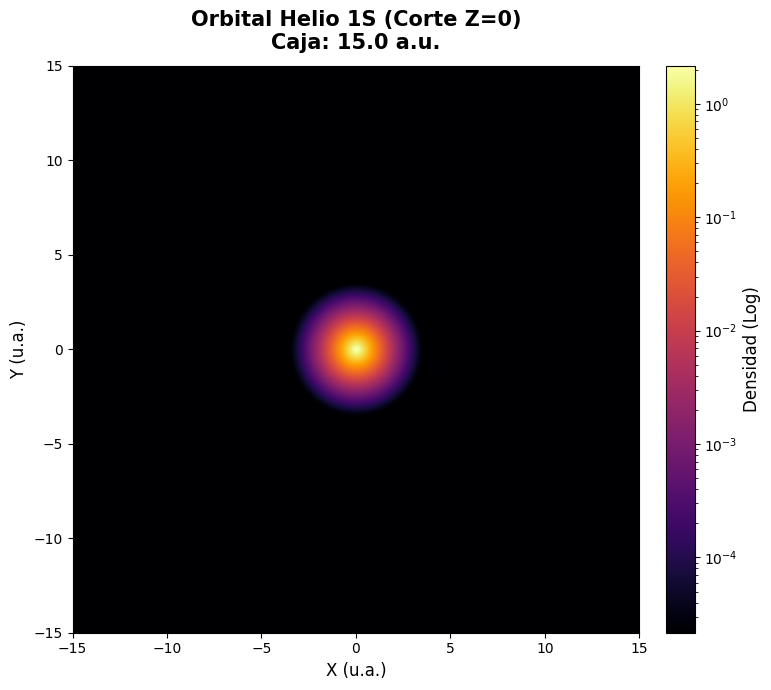
\includegraphics[width=0.45\textwidth]{1s.png}
    \caption{Sección transversal para el orbital $1s$ en unidades atómicas. El mapa de colores esta normalizado en torno al logaritmo del valor maximo para mejor visibilidad.}
    \label{fig:1s}
  \end{figure}

  \subsection{Energía de los estados excitados}

  Fue posible, haciendo uso de simetrias, encontrar los estados de mayor energia $2p_x$ y $3d_{x^2-y^2}$. Para el orbital $2p_x$ se obtuvo un valor de energía de $E^{obt}_{2p} = -19.093$ eV y para el orbital $3d_{x^2-y^2}$ el valor fue $E^{obt}_{3d} = -9.068$ eV

  \begin{figure}[h!]
    \centering
    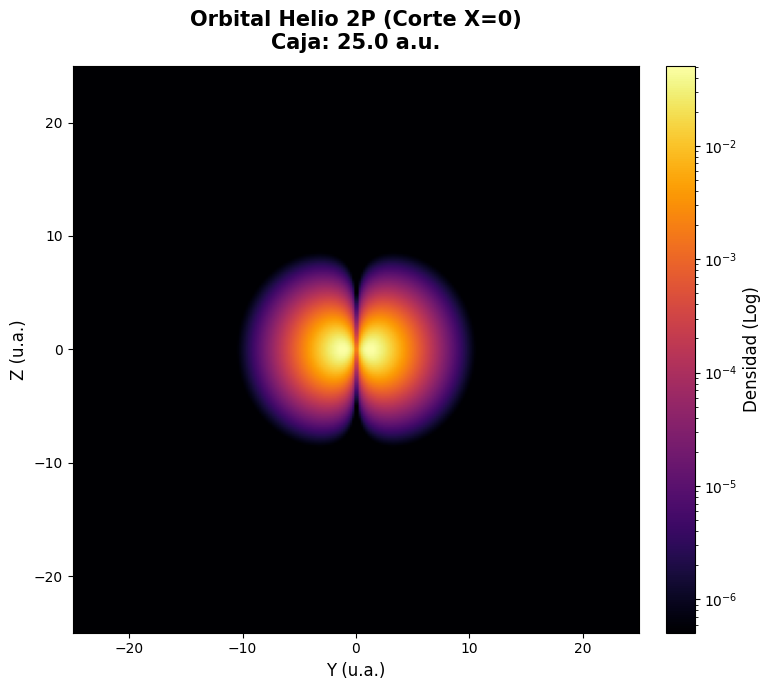
\includegraphics[width=0.45\textwidth]{2p.png}
    \caption{Sección transversal para el orbital $2p_x$ en unidades atómicas. Se puede apreciar la forma de la mancuerna dividida por un plano en z}
    \label{fig:2p}
  \end{figure}
  \begin{figure}[h!]
    \centering
    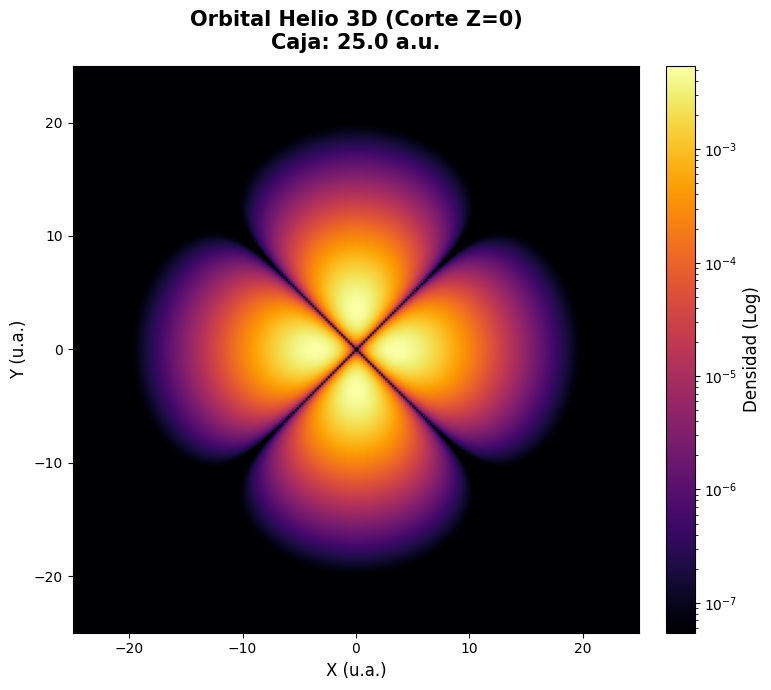
\includegraphics[width=0.45\textwidth]{3d.png}
    \caption{Sección transversal para el orbital $3d_{x^2-y^2}$ en unidades atómicas.Se puede apreciar la forma de trébol del orbital.}
    \label{fig:3d}
  \end{figure}

  \section{Discusión}

  \subsection{Precisión del valor de la energía del estado base}

  La discrepancia del $0.69\%$ en el valor respecto al límite teórico valida la estrategia numérica, aunque revela las limitaciones inherentes a la discretización. Este error residual se puede explicar en tres fuentes fundamentales, ordenadas por magnitud de impacto:

  \begin{enumerate}
    \item \textbf{Error espacial ($\Delta r$)}: La discretización finita del operador Laplaciano en la región nuclear introduce desviaciones. La función de onda 1s teórica presenta una singularidad en r=0. Al realizar una aproximación para evitar divergencias se pueden propagar desviaciones no deseadas, dando a lugar los resultados obtenidos. Esta se considera como la fuente dominante de discrepancia
    \item \textbf{Error temporal ($\Delta \tau$)}: El método Split-Operator introduce un error inherente debido a la aplicación de una expansion a segundo orden. El operador evolución trae asociado un error del orden $\mathcal{O}(\Delta\tau^3)$. Sin embargo, al utilizar un paso de tiempo $\Delta\tau = 10^{-4}$, esta fuente no realiza un aporte significativo.
    \item \textbf{Truncamiento del ciclo}: Si bien matemáticamente la convergencia del ciclo ocurre en el límite $\tau \to \infty$ al poner un limite en el numero de iteraciones el análisis de la evolución de la energía mostró estabilización antes de la iteración 60, por lo que el error asociado a detener la simulación en el paso 100 se puede despreciar.
  \end{enumerate}

  \subsection{Valores de energía de los estados excitados}

  Es fundamental interpretar correctamente los valores obtenidos. Dado que el método considera un valor de densidad de carga $\rho = 2|\phi|^2$, se está aplicando implícitamente el modelo Hartree-Fock Restringido (RHF). Esto implica que los estados excitados ($2p$,$3d$) no corresponden a las excitaciones de un solo electrón (ej. $1s12p1$) típicas, sino a estados doblemente excitados (ej. $2p2$, $3d2$) donde ambos electrones ocupan el mismo orbital superior. Esto explica por qué las energías calculadas se ven significativamente más altas que las del estado base.

  \subsection{Corrección de la auto-interacción en el potencial efectivo}

  La precisión obtenida no habría sido posible sin la corrección explícita de la auto-interacción en el potencial efectivo. Al escalar el término de repulsión por un factor de 0.5 en el Hamiltoniano efectivo ($V_{eff}=V_{nuc} + U^{eff}/2$), se logró que cada electrón "sintiera" únicamente el campo del otro electrón. Sin esta corrección, la energía calculada habría sido cercana a -40.815 eV (error $> 40\%$).

  \section{Conclusiones}

  En este proyecto se diseñó e implementó un simulador de primeros principios para la estructura electrónica del átomo de Helio aplicando el método de Hartree-Fock (SCF), utilizando programación en GPU utilizando C/CUDA.

  Se demostró que la combinación del método SCF con el de Propagación por Tiempo Imaginario (ITP) es una estrategia robusta y eficiente. Se logró reproducir la energía del estado fundamental del Helio con un valor de $E^{obt}_{1s} = -78.408$ eV, obteniendo un error relativo menor al $1\%$ respecto al límite teórico Hartree-Fock, $E^{HF} = -77.87$ eV.

  La implementación en C/CUDA permitió manejar mallas de alta resolución ($256^3\approx\ $ 16.7 millones de puntos) con tiempos de ejecución reducidos al paralelizar calculos directamente en la GPU, superando las limitaciones de las implementaciones secuenciales y/o paralelas tradicionales.

  Mediante la imposición de condiciones iniciales con simetría específica, el algoritmo fue capaz de converger permitiendo visualizar correctamente orbitales atómicos de mayor energía ($2p$, $3d$), revelando sus estructuras nodales características (mancuerna/trébol).

  Se verificó que, si bien el método es numéricamente preciso, está limitado físicamente por la aproximación de Hartree-Fock (ausencia de correlación electrónica) y el modelo RHF (estados doblemente excitados), lo cual debe ser considerado al comparar con datos experimentales.

  El proyecto demuestra la viabilidad y potencia de aplicar métodos en malla como alternativa a los métodos tradicionales de conjuntos de base empleando paralelización en GPU para resolver sistemas complejos de mecánica cuántica.

  \begin{thebibliography}{99}

% 1. Teoría Fundamental del Método ITP
\bibitem{lehtovaara}
L. Lehtovaara, J. Toivanen, and J. Eloranta, 
\textit{Solution of time-independent Schrödinger equation by spectral methods}, 
J. Comput. Phys. \textbf{221}, 148--157 (2007). 

% 2. La base matemática del Split-Operator (TU LINK DE ARXIV)
\bibitem{hatano_suzuki}
N. Hatano and M. Suzuki,
\textit{Finding Exponential Product Formulas of Higher Orders},
Lecture Notes in Physics \textbf{679}, 37--68 (2005).
[arXiv:math-ph/0506007].

% 4. Teoría de Hartree-Fock para Helio
\bibitem{udel_hf}
University of Delaware, 
\textit{Hartree-Fock Theory for Helium}, 
CHEM 444 Lecture Notes (2008). 
[Online]. Available: \url{https://www1.udel.edu/pchem/C444/spLectures/04222008b.pdf}

% 5. Datos Experimentales (NIST)
\bibitem{nist}
A. Kramida, Yu. Ralchenko, J. Reader, and NIST ASD Team (2024), 
\textit{NIST Atomic Spectra Database} (ver. 5.12), 
[Online]. Available: \url{https://physics.nist.gov/asd}.

\end{thebibliography}
  \end{document}
